\chapter{Getting Started} \label{ch:gettingStarted}

\section{Installation} \label{sec:installation}

\vvase{} does not include any installation process or changes to the machine registry.  Simply place the executable and the pdf manual into the same directory.  After running the first time, any changes to the default settings are saved to a configuration file which will appear in the directory from which the application is run.

\section{Overview} \label{sec:overview}

Upon starting \vvase{} for the first time, the screen will look like \figref{fig:defaultStartup}.  Counter-clockwise from the top left corner of the window are the \element{Systems Tree} (\sref{ssec:systemsTree}), \element{Edit Panel} (\sref{ssec:editPanel}), \element{Output Pane} (\sref{ssec:outputPane}), \element{Output List} (\sref{ssec:outputList}) and \element{Main Display Area} (\sref{ssec:mainDisplayArea}).  Above these elements are two toolbars, the \element{Kinematics Toolbar} (\sref{ssec:kinematicsToolbar}) and the \element{3D Toolbar} (\sref{ssec:3DToolbar}).  Across the top of the window is a typical menu bar, the contents of which are described in \sref{ssec:menuBar}.  All of these elements can be dragged, floated or docked to create the desired layout.

\begin{figure}
  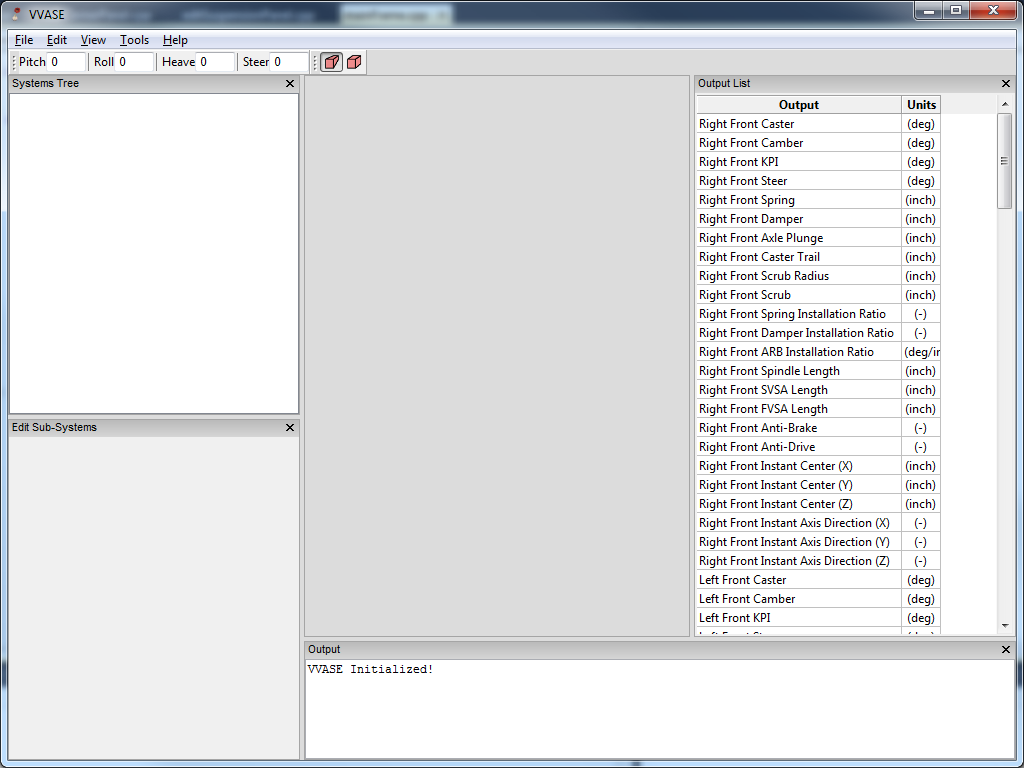
\includegraphics[width=\textwidth]{images/defaultStartup}
  \caption{Default screen configuration} \label{fig:defaultStartup}
  \centering
\end{figure}

\subsection{Systems Tree} \label{ssec:systemsTree}

The \element{Systems Tree} lists all of the files that are currently open.  Some files include sub-items which can be accessed by expanding the parent item.  Right-clicking on \element{Systems Tree} entries results in a context menu from which files can be saved or closed.

\subsection{Edit Panel} \label{ssec:editPanel}

The \element{Edit Panel} is where the core modifications to all files are made.  When a file is selected by either selecting its tab in the \element{Main Display Area} or clicking on it in the \element{Systems Tree}, the \element{Edit Panel} changes to show options relevant to the selected file.  For files that include sub-items in the \element{Systems Tree}, each sub-item may have different editable parameters.

\subsection{Output Pane} \label{ssec:outputPane}

The \element{Output Pane} primarily contains diagnostic output to inform the user about problems encountered while computing the kinematics.  For example, if a kinematic state is specified that would result in the suspension reaching its droop limit, the solver will be unable to solve for some of the hardpoint locations.  Depending on how verbose the messages are configured to be (see \sref{ssec:optionsDebugging}), the user will be notified that there was a problem computing the solution for one corner of the car or exactly which hardpoint it was that presented a problem.

\subsection{Output List} \label{ssec:outputList}

The \element{Output List} contains a complete listing of all of the computed kinematic outputs for all open car files for the specified kinematic state (see \sref{ssec:kinematicsToolbar}).  The computed outputs are listed in rows and the open car files are listed in columns.  This arrangement makes side-by-side comparisons of kinematic outputs for multiple car files very easy.  When an output is undefined (e.g. when the kinematic roll center crosses the ground plane), the corresponding grid cell is highlighted yellow and the text ``Undef.'' is displayed in the cell.  If an output doesn't apply for a certain car file (e.g. front-wheel axle plunge on a rear-wheel drive car), the text ``N/A'' is displayed.

\subsection{Main Display Area} \label{ssec:mainDisplayArea}

The \element{Main Display Area} is a tabbed window and contains a tab for each open file.  Each file type contains a unique display.  Car files show a 3D image of the vehicle in the specified kinematic state (see \sref{ch:cars}), iteration files show a 2D plot showing calculated kinematic outputs across a range of kinematic states (see \sref{ch:iterations} and optimizations show a set of controls that allow configuration of the optimization parameters (see \sref{ch:optimizations}).

The tabs in this area can be dragged, docked or floated to enable viewing the 3D model of the car adjacent to an iteration plot, or multiple iteration plots simultaneously.  See \figref{fig:multiPlot} for an example.

\begin{figure}
  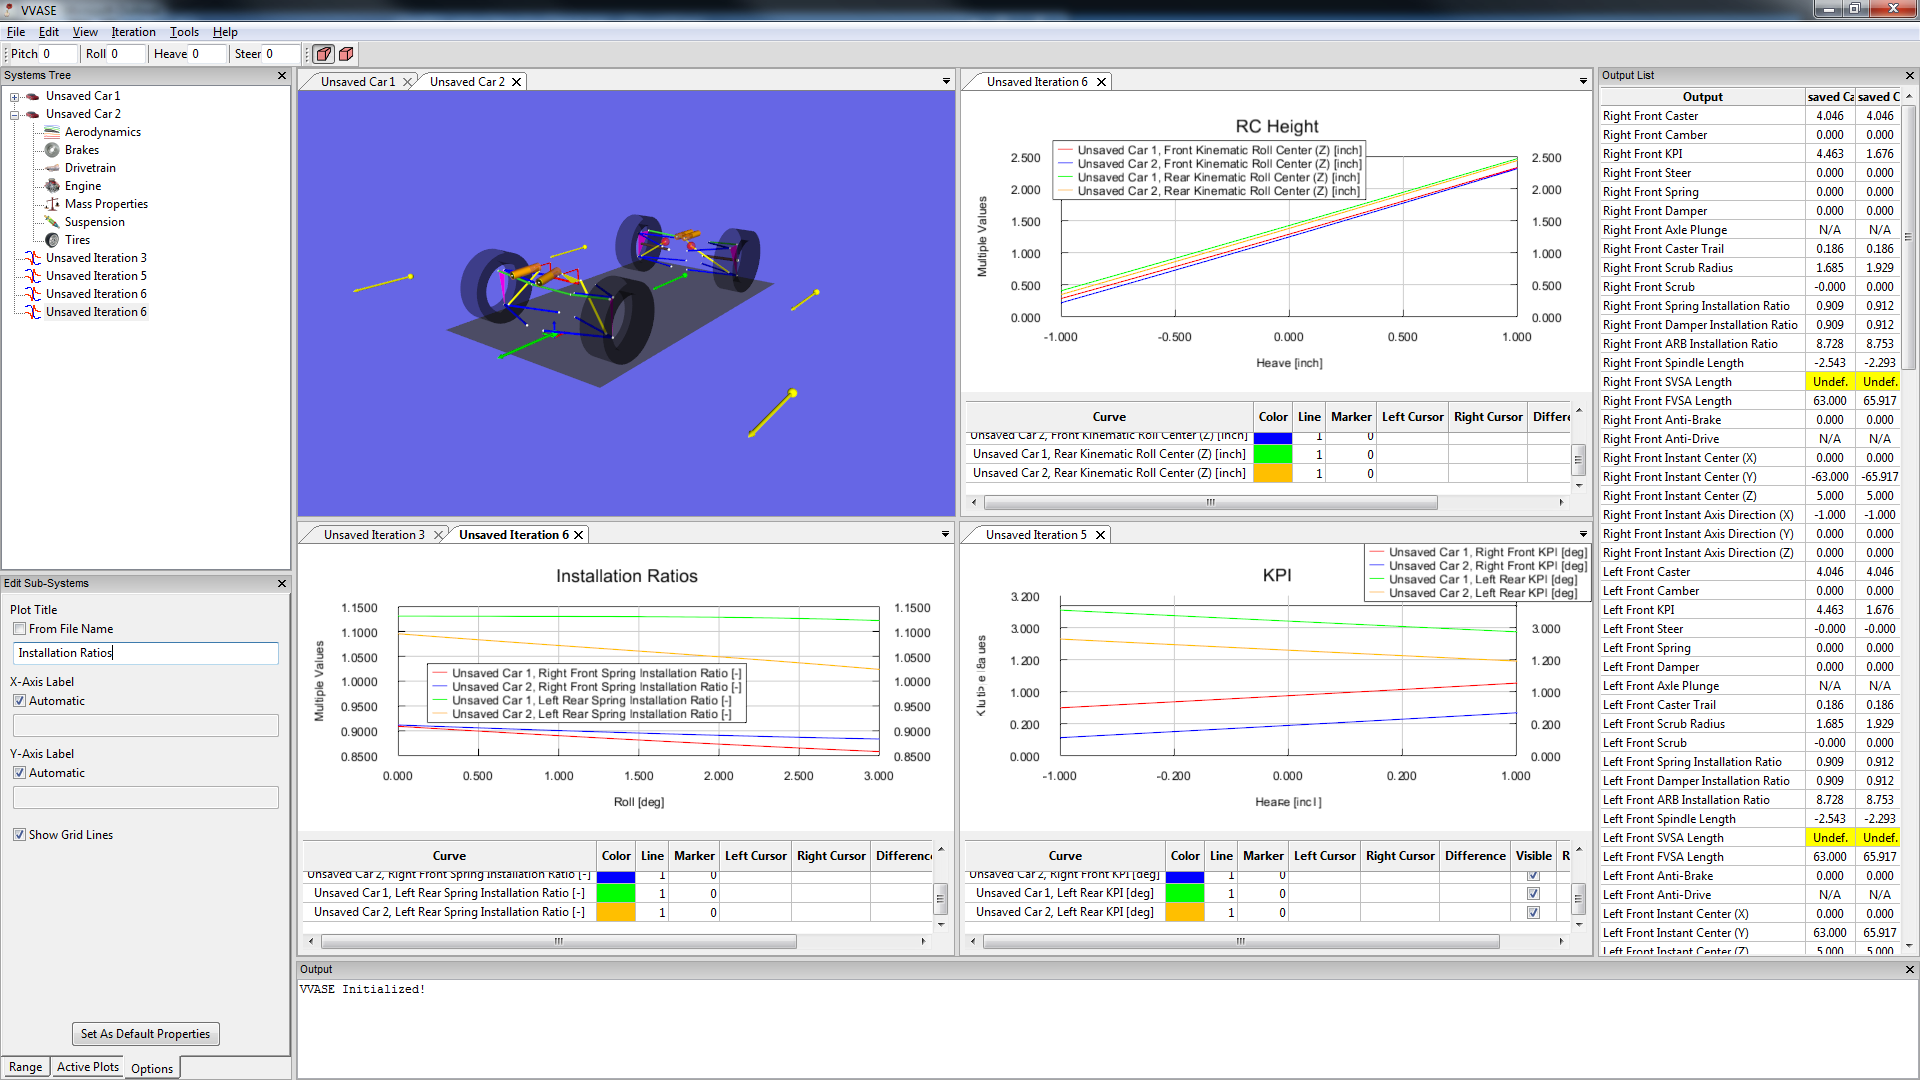
\includegraphics[width=\textwidth]{images/multiPlot}
  \caption{Custom layout demonstrating multiple plots displayed simulatenously} \label{fig:multiPlot}
  \centering
\end{figure}

\subsection{Kinematics Toolbar} \label{ssec:kinematicsToolbar}

The \element{Kinematics Toolbar} is where the user can define a kinematic state for which the kinematic outpus shall be calculated.  As the user types in the Pitch, Roll, Heave and Steer boxes, the kinematic outputs are computed for all open car files and the \element{Main Display Area} and \element{Output Lists} are updated.  The units for these inputs are determined by the options set in the options dialog (see \sref{ssec:optionsUnits}).

\subsection{3D Toolbar} \label{ssec:3DToolbar}

The \element{3D Toolbar} only affects the \element{Main Display Area} for car files.  There are two toggle buttons which switch between perspective and orthographic view modes.  Perspective mode draws objects in the foreground with a larger scale than objects in the background (the way objects appear in the real world).  Orthographic mode draws all objects at the same scale.  While perspective mode tends to be more pleasing, orthographic view can be helpful for example when visually determining how well points on opposite ends of the car line up.

\subsection{Menu Bar} \label{ssec:menuBar}

The application Menu Bar is fairly self explanatory.  The \element{File} menu permits saving, loading and closing files.  The \element{Edit} menu contains entries for undo/redo and cut/copy/paste.  The \element{View} menu gives the user some control over the display of toolbars and the \element{Output Pane} contents.  The \element{Tools} menu includes an item to display the \element{Options Dialog} (see \sref{sec:options}.  The \element{Help} menu includes a link to open this document and can display information about \vvase{}.

Depending on what type of file is active, there may be an additional menu entry with specific options pertaining to the active file.

\section{Options} \label{sec:options}

In addition to display customization, there are several ways in which the behavior of \vvase{} can be adjusted to suit user preferences.  All preferences are automatically saved when \vvase{} exits and loaded each time it starts.

\subsection{Units} \label{ssec:optionsUnits}

\vvase{} allows the user to specify which units to use for each type of unit.  After selections are made and changes are applied, all inputs and outputs are updated to be consistent with the specified units.  The options tab containing the units options is shown in \figref{fig:optionsUnits}.

\begin{figure}
  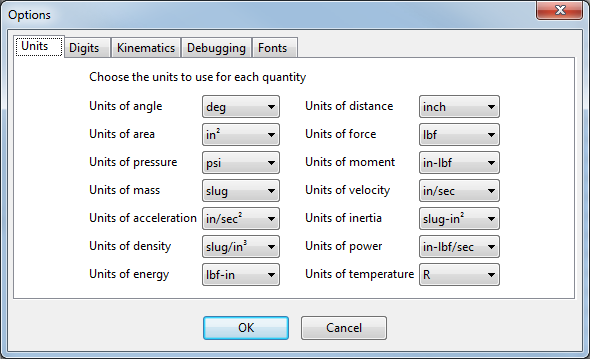
\includegraphics[width=\textwidth]{images/optionsUnits}
  \caption{Units options} \label{fig:optionsUnits}
  \centering
\end{figure}

\subsection{Digits} \label{ssec:optionsDigits}

If desired, the precision with which values are displayed can be adjusted.  Optionally, value can also be displayed in scientific notation or while preserving a constant number of significant digits.  The options tab containing the digits options is shown in \figref{fig:optionsDigits}.

\begin{figure}
  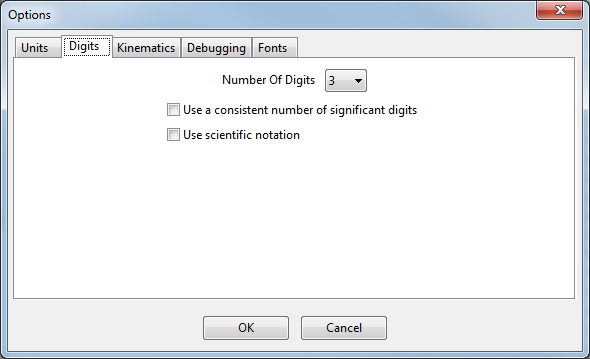
\includegraphics[width=\textwidth]{images/optionsDigits}
  \caption{Digits options} \label{fig:optionsDigits}
  \centering
\end{figure}

\subsection{Kinematics} \label{ssec:optionsKinematics}

When applying the specified kinematic state to the car, \vvase{} applies the rotations about the center of rotation specified here.  The default location of $\left(0, 0, 0\right)$ is probably fine for applying roll motion, but when applying pitch, the default center of rotation is likely to result in excessive vertical displacement at the rear end.  This can be resolved by moving the center of rotation backwards.

A frequently asked question is ``why doesn't the center of rotation match the roll center?''  The answer is that cars do not roll about the roll center.  Since tires and springs (and dynamically, dampers) are involved, the actual instantaneous location of the vehicle's rolling motion is the result of the forces acting on the components of the vehicle.  Since the kinematics model does not include any forces, no attempt is made to compute the actual attitude that a car would reach during dynamic or even steady-state conditions.  Instead, \vvase{} answers the question ``if the car were to attain this attitude, what are the values of the relevant kinematic outputs?''

Additionally, the order in which the pitch and roll rotations are applied can be changed.

The ``Steering Input'' option allows the user to specify how the Steer input should be interpreted.  In the case of ``Use rack travel distance,'' the input is interpreted as a distance and applied directly to the locations of the inboard tie rods.  In the case of ``Use steering wheel angle,'' the input is interpreted as an angle, and converted to linear motion of the steering rack according to the specified steering ratio.

The number of threads to execute is generated by estimating the value that would make most efficient use of the available CPU cores.  For large optimizations, it may be desirable to fine-tune this value in order to ensure the best possible performance.

The options tab containing the kinematics options is shown in \figref{fig:optionsKinematics}.

\begin{figure}
  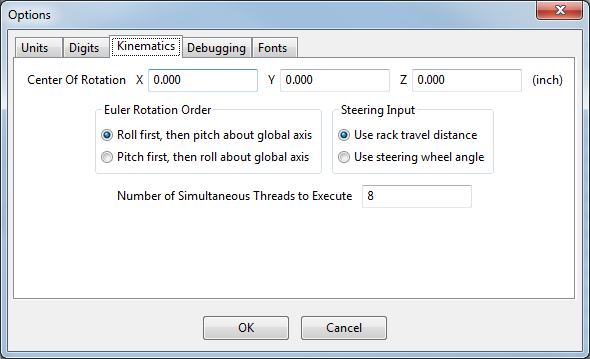
\includegraphics[width=\textwidth]{images/optionsKinematics} \label{fig:optionsKinematics}
  \caption{Kinematics options}
  \centering
\end{figure}

\subsection{Debugging} \label{ssec:optionsDebugging}

The debugging options apply to the messages that appear in the \element{Output Pane}.  Generally, the default level (Normal) is ideal, however in the event that a particular suspension is not properly solving, it can be helpful to make the debug level more verbose.  The options tab containing the debugging options is shown in \figref{fig:optionsDebugging}.

\begin{figure}
  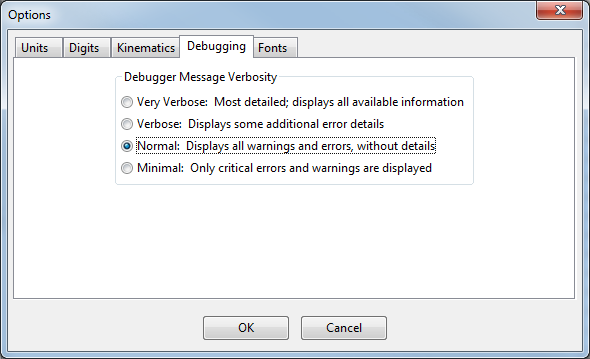
\includegraphics[width=\textwidth]{images/optionsDebugging}
  \caption{Debugging options} \label{fig:optionsDebugging}
  \centering
\end{figure}

\subsection{Fonts} \label{ssec:optionsFonts}

If desired, the fonts used for rendering the iteration plots and the font used for printing to the Output Pane can be changed.  For best results, it is recommended to only select TrueType fonts for use with the iteration plots.  The options tab containing the fonts options is shown in \figref{fig:optionsFonts}.

\begin{figure}
  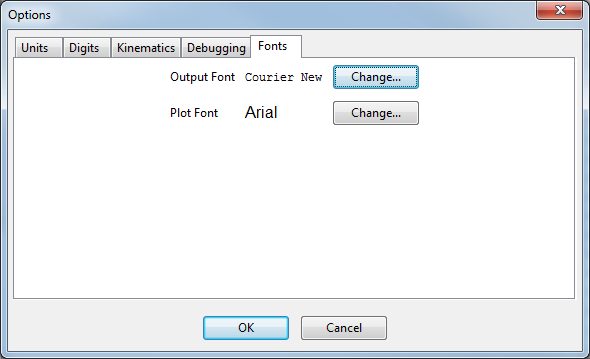
\includegraphics[width=\textwidth]{images/optionsFonts}
  \caption{Fonts options} \label{fig:optionsFonts}
  \centering
\end{figure}
